% document class using the Springer publishing company's document class
\documentclass[envcountsame,envcountchap]{svmono}

% packages to include additional functionality
\usepackage{makeidx}         % allows index generation
\usepackage{graphicx}        % standard LaTeX graphics tool
                             % when including figure files
\usepackage{multicol}        % used for the two-column index
\usepackage[bottom]{footmisc}% places footnotes at page bottom
\usepackage{wrapfig} % for wrapping images with text
\usepackage{color} % for coloring links
\usepackage{fancyvrb}
\usepackage{listings}
\usepackage{capt-of}
\usepackage{fixltx2e}
\usepackage{hyperref}
\hypersetup{colorlinks=false}


\begin{document}

\author{Khaja Masroor Ahmed}
\title{Assignment 2}

\subtitle{CS 751:  Introduction to Digital Libraries\\Dr. Michael Nelson\\Spring 2015}

% note that this special command is part of the document class
% and, in addition to creating the title page, also inserts the 
% current date on the page
\maketitle

\frontmatter

\tableofcontents

\mainmatter

% include other tex files so we don't have one huge document to scroll through
\chapter{Question 1}
\label{question-1}
\section{Question}

\begin{itemize}
\item For the text you saved for the 10000 URIs from A1, Q2:
	\begin{itemize}
	\item Use the “boilerpipe” software to remove the HTML templates from all HTML pages (document how many pages link from the tweets were non-HTML and had to be skipped).
	\item \url{https://code.google.com/p/boilerpipe/}
	\item WSDM 2010 paper: \url{http://www.l3s.de/~kohlschuetter/boilerplate/}
	\end{itemize}
\item For how many of the 10000 URIs was boilerpipe successful?
	\begin{itemize}
	\item Compare the total words, unique words, and byte sizes before and after use of boilerpipe.
	\end{itemize}
\item For what classes of pages was it successful?
\item For what classes of pages was it unsuccessful?
\item Provide examples of both successful and unsuccessful removals and discuss at length.
\end{itemize}


\section{Solution}
\begin{itemize}
\item For this assignment I used the boilerpipe library on python.
\item I installed the library on the linux machine using the command `sudo pip install boilerpipe'.
\item I saved the HTML files that I downloaded from the first assignment to my folder located at \url{www.cs.odu.edu/~kahmed/cs751/a3/} so I could use them as URIs to be used for the boilerpipe script.
\item From the 10000 URIs I was able to download the HTML files for 9978 URIs. The files were not created for the URIs which returned a 404 response. From the remaining URIs I was able to retrieve 8476 URIs as some of them did not have any HTML data.
\item From the 8476 URIs that remained after successful retrieval of HTML content, the boilerpipe was successful for 6275 URIs. Below is a comparison of the data before and after running them through the boilerpipe script. \\*
	\begin{minipage}{\linewidth}
		\centering
			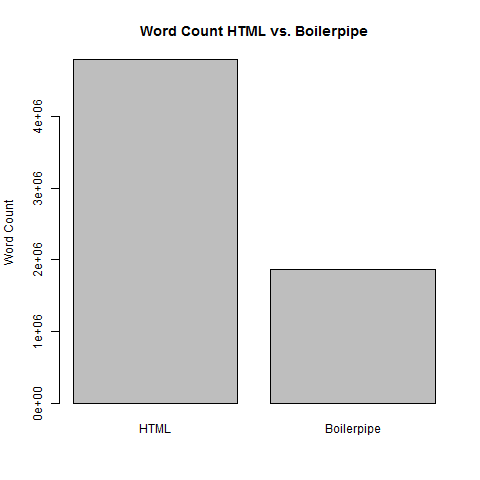
\includegraphics[scale=0.55]{figures/wordCount.png}
		\captionof{figure}{Word Count for HTML vs. Boilerpipe}
		\label{wordCount}
	\end{minipage}
	\begin{minipage}{\linewidth}
		\centering
			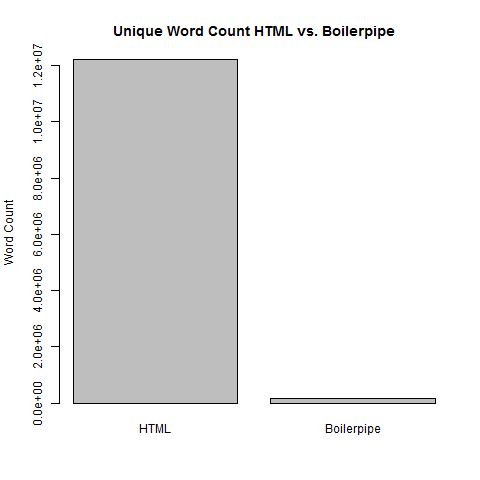
\includegraphics[scale=0.55]{figures/uniqueWord.png}
		\captionof{figure}{Unique Word Count for HTML vs. Boilerpipe}
		\label{uniqueWord}
	\end{minipage}
	\begin{minipage}{\linewidth}
		\centering
			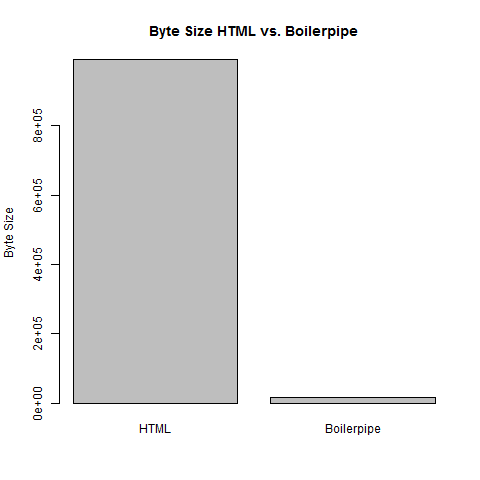
\includegraphics[scale=0.55]{figures/byteSize.png}
		\captionof{figure}{Byte Size for HTML vs. Boilerpipe}
		\label{byteSize}
	\end{minipage}
\item I used python scripts to retrieve this information for individual files and then used Microsoft Excel to get the total number of words in each case.
\end{itemize}

\subsection{Boilerpipe Successful}
\begin{itemize}
\item I selected a few URIs for which the boilerpipe was successful.
\item A few examples of successful boilerpipe retrieval are:
	\begin{itemize}
	\item \url{http://her-life-and-health.com/?a=adm}
	\item \url{https://play.google.com/store/apps/details?id=com.maoline.kindan.droid}
	\end{itemize}
\item I noticed that the successful ones had HTML elements such as `<div>', `<p>', etc. with text enclosed within them.
\end{itemize}

\subsection{Boilerpipe Unsuccessful}
\begin{itemize}
\item I performed the same activity of selecting URIs for which boilerpipe was unsuccessful.
\item A few examples of unsuccessful boilerpipe retrieval are:
	\begin{itemize}
	\item \url{http://jsm084.wix.com/joy1063}
	\item \url{http://instagram.com/p/ysl6lgFD_H/}
	\end{itemize}
\item Upon further investigation of these HTML pages, I came to a conclusion that the HTML pages for these URIs had only HTML script tags such as `<script>' within them.
\item The boilerpipe is designed the ignore the data enclosed within these script tags.
\item It is designed to check for data enclosed within the block elements like `<div>', '<p>', etc.
\item For the example listed above, the Instagram URI ran external scripts for fetching the data to be displayed. The HTML page basically consists of scripts to be called and the necessary arguments to be passed to the script to display the necessary content which in this case was a picture and the comments for that picture from other Instagram users.
\item This is applicable for the rest of the URIs for which boilerpipe was unsuccessful.
\end{itemize}

\newpage
\section{Code Listing}

\lstinputlisting[language=Python,breaklines = true,frame=single,caption={Python program for retrieving the boilerpipe data.},label=lst:q1-1,captionpos=b,numbers=left,showspaces=false,showstringspaces=false,basicstyle=\footnotesize]{pythonFiles/boilerPipe.py}
\newpage
\lstinputlisting[language=Python,breaklines = true,frame=single,caption={Python program for retrieving the unique word count from HTML.},label=lst:q1-1,captionpos=b,numbers=left,showspaces=false,showstringspaces=false,basicstyle=\footnotesize]{pythonFiles/readHtml.py}
\newpage
\lstinputlisting[language=Python,breaklines = true,frame=single,caption={Python program for retrieving the word count for individual file.},label=lst:q1-1,captionpos=b,numbers=left,showspaces=false,showstringspaces=false,basicstyle=\footnotesize]{pythonFiles/wordCount.py}
\newpage
\lstinputlisting[language=Python,breaklines = true,frame=single,caption={Python program for retrieving unique word list for boilerpipe successful files.},label=lst:q1-1,captionpos=b,numbers=left,showspaces=false,showstringspaces=false,basicstyle=\footnotesize]{pythonFiles/wordList.py}

\newpage
\lstinputlisting[language=R,breaklines = true,frame=single,caption={R program for generating the bar plot for total word count for HTML vs. Boilerpipe}, label=lst:q1R1,captionpos=b,numbers=left,showspaces=false,showstringspaces=false,basicstyle=\footnotesize]{rFiles/wordCount.R}
\lstinputlisting[language=R,breaklines = true,frame=single,caption={R program for generating the bar plot for unique word count for HTML vs. Boilerpipe}, label=lst:q1R1,captionpos=b,numbers=left,showspaces=false,showstringspaces=false,basicstyle=\footnotesize]{rFiles/uniqueWord.R}
\lstinputlisting[language=R,breaklines = true,frame=single,caption={R program for generating the bar plot for byte size of HTML vs. Boilerpipe}, label=lst:q1R1,captionpos=b,numbers=left,showspaces=false,showstringspaces=false,basicstyle=\footnotesize]{rFiles/byteSize.R}
\chapter{Question 2}
\label{question-2}
\section{Question}



\begin{itemize}
\item Collection1: Extract all the unique terms and their frequency from the 10000 files{*}.
\item Collection2: Extract all the unique terms and their frequency of the 10000 files{*} after running boilerpipe.
\item Construct a table with the top 50 terms from each collection. 
	\begin{itemize}
	\item Find a common stop word list.  How many of the 50 terms are on that stop word list?
	\end{itemize}
\item For both collections, construct a graph with the x-axis as word rank, and y-axis as word frequency.
	\begin{itemize}
	\item Do either follow a Zipf distribution? Support your answer.
	\end{itemize}	
\end{itemize}

\section{Solution}

\begin{itemize}
\item I ordered the word list that I received as an output from the previous question and then got the highest frequency word list.
\item I fetched the stop word list by searching for it on \url{www.google.com} and then compared the top 50 results with the stop word list.
\item For HTML files before running boilerpipe, there were 43 common words with the stop word list.
\item After running boilerpipe, there were 44 common words with the stop word list.
\item Below are tables indicating the results for the high frequency word list for HTML and boilerpipe.
\end{itemize}

\begin{table}

\caption{Collection 1: Word Rank and Frequency before boilerpipe}
\begin{center}
\begin{tabular}{ c | c | c | c}
\hline
Rank & Word & Frequency & Stop Word \\ \hline

1 & a & 484037 & Yes \\ \hline
2 & the & 137978 & Yes \\ \hline
3 & to & 115694 & Yes \\ \hline
4 & and & 96843 & Yes \\ \hline
5 & in & 73996 & Yes \\ \hline
6 & of & 70699 & Yes \\ \hline
7 & for & 49243 & Yes \\ \hline
8 & on & 44144 & Yes \\ \hline
9 & this & 38794 & Yes \\ \hline
10 & is & 38490 & Yes \\ \hline
11 & with & 37402 & Yes \\ \hline
12 & by & 34809 & Yes \\ \hline
13 & you & 33828 & Yes \\ \hline
14 & your & 33537 & Yes \\ \hline
15 & that & 21535 & Yes \\ \hline
16 & all & 20933 & Yes \\ \hline
17 & from & 19210 & Yes \\ \hline
18 & it & 18456 & Yes \\ \hline
19 & at & 18300 & Yes \\ \hline
20 & are & 17710 & Yes \\ \hline
21 & be & 17238 & Yes \\ \hline
22 & or & 15885 & Yes \\ \hline
23 & as & 15391 & Yes \\ \hline
24 & will & 15035 & Yes \\ \hline
25 & important & 14690 & No \\ \hline
26 & no & 13703 & Yes \\ \hline
27 & an & 12070 & Yes \\ \hline
28 & was & 12054 & Yes \\ \hline
29 & more & 12026 & Yes \\ \hline
30 & have & 11805 & Yes \\ \hline
31 & do & 11350 & Yes \\ \hline
32 & about & 9915 & Yes \\ \hline
33 & out & 9791 & Yes \\ \hline
34 & arabic word & 9647 & No \\ \hline
35 & right & 9459 & No \\ \hline
36 & we & 9303 & Yes \\ \hline
37 & our & 9213 & Yes \\ \hline
38 & has & 9100 & Yes \\ \hline
39 & my & 8601 & Yes \\ \hline
40 & l & 8579 & Yes \\ \hline
41 & one & 8271 & No \\ \hline
42 & only & 8162 & Yes \\ \hline
43 & me & 7560 & Yes \\ \hline
44 & can & 7497 & No \\ \hline
45 & but & 7480 & Yes \\ \hline
46 & he & 7264 & Yes \\ \hline
47 & his & 7163 & Yes \\ \hline
48 & when & 7124 & Yes \\ \hline
49 & arabic word & 6946 & No \\ \hline
50 & us & 6914 & No \\ \hline
\hline

\end{tabular}
\end{center}
\end{table} ​

\begin{table}
\caption{Collection 2: Word Rank and Frequency after boilerpipe}
\begin{center}
\begin{tabular}{ c | c | c | c}
\hline
Rank & Word & Frequency & Stop Word \\ \hline

1 & the & 54339 & Yes \\ \hline
2 & to & 35095 & Yes \\ \hline
3 & a & 32042 & Yes \\ \hline
4 & and & 30095 & Yes \\ \hline
5 & of & 24486 & Yes \\ \hline
6 & in & 18309 & Yes \\ \hline
7 & is & 14296 & Yes \\ \hline
8 & you & 12979 & Yes \\ \hline
9 & play & 12961 & No \\ \hline
10 & for & 11707 & Yes \\ \hline
11 & that & 11592 & Yes \\ \hline
12 & this & 11315 & Yes \\ \hline
13 & on & 10768 & Yes \\ \hline
14 & i & 9818 & Yes \\ \hline
15 & it & 9112 & Yes \\ \hline
16 & now & 8817 & Yes \\ \hline
17 & with & 8687 & Yes \\ \hline
18 & your & 8444 & Yes \\ \hline
19 & next & 7133 & No \\ \hline
20 & by & 6724 & Yes \\ \hline
21 & are & 6502 & Yes \\ \hline
22 & as & 6414 & Yes \\ \hline
23 & be & 6114 & Yes \\ \hline
24 & have & 5681 & Yes \\ \hline
25 & was & 5613 & Yes \\ \hline
26 & or & 5553 & Yes \\ \hline
27 & not & 5477 & Yes \\ \hline
28 & at & 4937 & Yes \\ \hline
29 & from & 4894 & Yes \\ \hline
30 & we & 4758 & Yes \\ \hline
31 & no & 4727 & Yes \\ \hline
32 & more & 4588 & Yes \\ \hline
33 & has & 4064 & Yes \\ \hline
34 & but & 3994 & Yes \\ \hline
35 & an & 3969 & Yes \\ \hline
36 & all & 3781 & Yes \\ \hline
37 & will & 3780 & No \\ \hline
38 & they & 3587 & Yes \\ \hline
39 & can & 3585 & Yes \\ \hline
40 & if & 3272 & Yes \\ \hline
41 & he & 3263 & Yes \\ \hline
42 & up & 3260 & No \\ \hline
43 & about & 3243 & Yes \\ \hline
44 & do & 3084 & Yes \\ \hline
45 & arabic word & 3040 & No \\ \hline
46 & our & 3010 & Yes \\ \hline
47 & when & 2943 & Yes \\ \hline
48 & my & 2875 & Yes \\ \hline
49 & been & 2839 & Yes \\ \hline
50 & arabic word & 2755 & No \\ \hline
\hline

\end{tabular}
\end{center}
\end{table} ​


	\begin{minipage}{\linewidth}
		\centering
			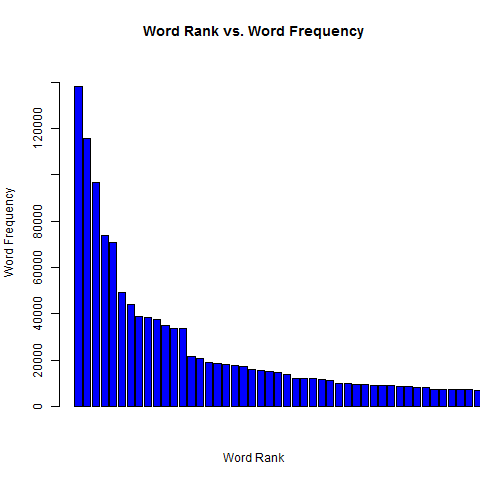
\includegraphics[scale=0.55]{figures/beforeBP.png}
		\captionof{figure}{Distribution of data for high frequency words before boilerpipe.}
		\label{wordCount}
	\end{minipage}
	\begin{minipage}{\linewidth}
		\centering
			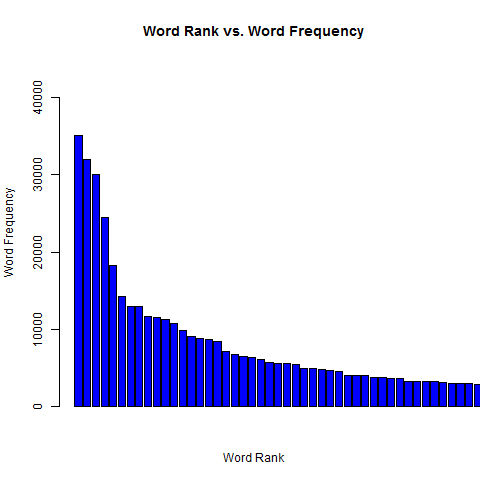
\includegraphics[scale=0.55]{figures/afterBP.png}
		\captionof{figure}{Distribution of data for high frequency words after boilerpipe.}
		\label{wordCount}
	\end{minipage}
\begin{itemize}
\item The above graphs indicate that they follow the zipf distribution as the word rank is inversely proportional to its frequency.
\end{itemize}

\newpage
\section{Code Listing}

\lstinputlisting[language=R,breaklines = true,frame=single,caption={R program for generating the bar plot for high frequency words before boilerpipe.}, label=lst:q1R1,captionpos=b,numbers=left,showspaces=false,showstringspaces=false,basicstyle=\footnotesize]{rFiles/beforeBP.R}
\lstinputlisting[language=R,breaklines = true,frame=single,caption={R program for generating the bar plot for high frequency words after boilerpipe.}, label=lst:q1R1,captionpos=b,numbers=left,showspaces=false,showstringspaces=false,basicstyle=\footnotesize]{rFiles/afterBP.R}
\backmatter

% include other tex files
\bibliographystyle{plain}
\bibliography{reference}
\nocite{*}

\end{document}